\nsecbegin{Was wird wie gemacht?}
\nsecbegin{Eclipse}
\nsecbegin{Projekt in Eclipse importieren}
In den workspace wecheln:\\
cd ~/workspace\\
Projekt Klonen:\\
git clone https://gitlab.imn.htwk-leipzig.de/weicker/puml.git\\
Benutzername und Passwort eingeben.\\
In Eclipse "File->Import->Existing Projects into Workspace"\\
%\begin{figure}[hbtp]
%\centering
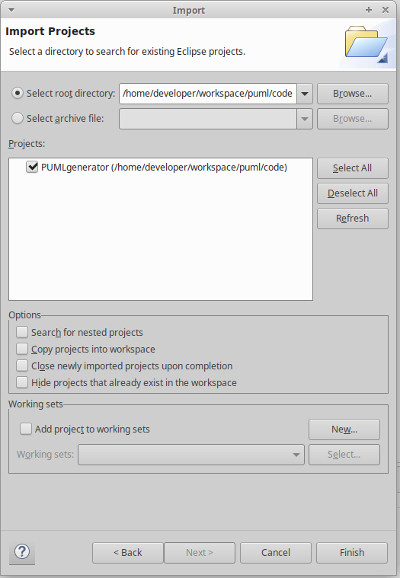
\includegraphics[scale=0.25]{Bilder/importProject}\\
%\caption{Projekt in Eclipse importieren}
%\end{figure}
Dann auf "'Finish"' klicken.
\nsecend

\nsecbegin{WindowBuilder installieren}
In Eclipse "Help->Install New Software..."\\
Unter work with "'2018-09 - http://download.eclipse.org/releases/2018-09"' auswählen.\\
In der Section "'General Purpose Tools"' die im Bild stehenden Häckchen anklicken\\	
\begin{figure}[hbtp]
\centering
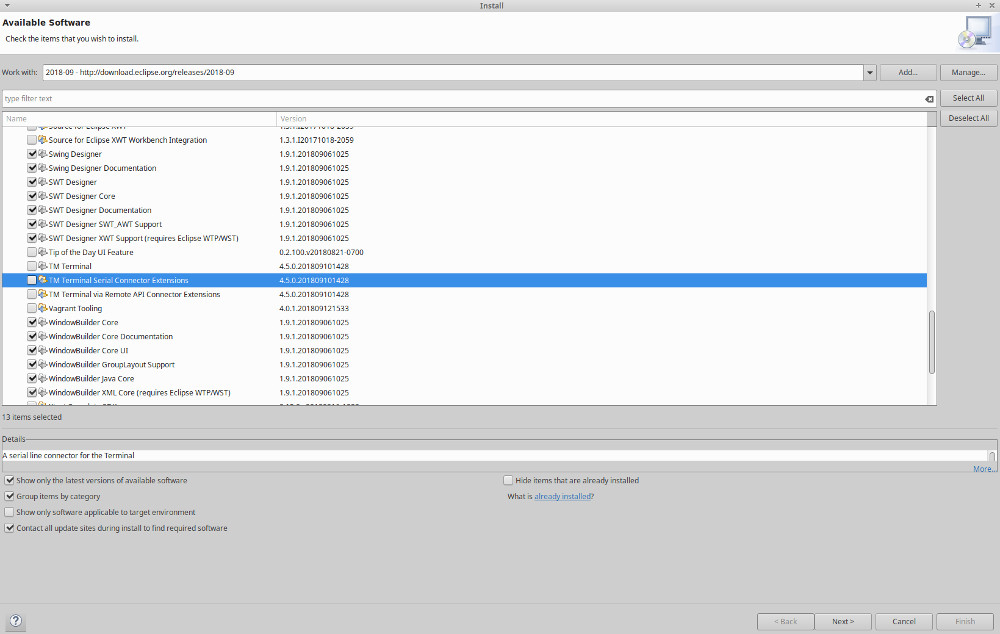
\includegraphics[scale=0.4]{Bilder/installWindowBuilder}\\
\caption{WindowBuilder installieren}
\end{figure}
Dann auf "'Finish"' und sich durch die Installation klicken.
\nsecend

\nsecbegin{GUI editieren}
Es muss der WindowBuilder installiert sein. Dann auf die Datei die die Grafische Oberfläche implementiert (GUI.java) mit der rechten Maustaste klicken. Dann "'Open With->WindowBuilder Editor"' auswählen.
\nsecend
\nsecend %{Eclipse}

\nsecbegin{LaTeX}
\nsecbegin{Geschachtelte Überschriften}
Durch die Makros:
\begin{itemize}
\item \textbackslash nsecbegin\{MeineÜberschrift\}
\item \textbackslash nsecend
\end{itemize}
können geschachtelte Überschriften verwendet werden. Die Kapitel einfach in diese Makros einschließen. Somit muss nicht darauf geachtet werden auf welcher Ebene man sich im Moment befindet. Dies vereinfacht insbesondere das Auslagern von Text in andere Dateien.\\
Um die Makros in die Autovervollständigung des Texmakers aufzunehmen "'Benutzer/in->Wortvervollständigung anpassen"' wählen und dort die Makros hinzufügen.
\begin{figure}[hbtp]
\centering
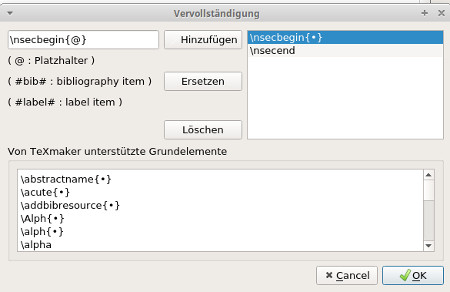
\includegraphics[scale=0.4]{Bilder/autocompleteMakro}
\caption{Autovervollständigung anpassen}
\end{figure}
\nsecend

\nsecbegin{Build-Dateien aufräumen}
Beim erstellen des LaTeX-Dokuments werden jede Menge zusätzliche Dateien erstellt. Dank der entsprechenden "'.gitignore-Datei"' werden diese nicht in GIT hinzugefügt. Für den Fall dass man das Verzeichniss bei sich selbst bereinigen möchte, kann das "'clean.sh"'-Script ausgeführt werden.
\nsecend

\nsecbegin{Entwicklerdokumentation und Handbuch erstellen}
Wenn etwas an der Entwicklerdokumentation oder am Handbuch geändert wurde, müssen diese Dokumente neu erstellt werden. Hierfür zunächst wie gewohnt die LaTeX-Projektdokumentation erstellen. Anschließend kann das "'buildAllDocuments.sh"'-Script ausgeführt werden. Dieses erstellt dann die entsprechenden Dokumente.\\
Weitere Informationen zum "'multiaudience-Paket"' unter \url{https://www.uweziegenhagen.de/?p=3252}.
\nsecend
\nsecend %{Latex}


\nsecbegin{GIT}

\nsecbegin{Benutzername und eMail ins GIT eintragen}
In Linux kann durch den Aufruf:\\
gedit \textasciitilde /.gitconfig\\
die "'.gitconfig-Datei"' editiert werden. In dieser werden unter anderem auch Benutzername und eMail-Addressse des Benutzers gespeichert.
\nsecend

\nsecbegin{Basics}
\begin{lstlisting}[language=bash]
#Aktueller Zustand ausgeben
#Auf Welchem Branch bin ich?
#Gibt es Dateien die geändert sind? 
#Wurden Dateien gelöscht? 
#Wurden neue Dateien hinzugefügt?
#Sind Aenderungen bereits für den Commit vorgemerkt?
#Bin ich vor oder hinter dem Remote-branch?
git status

#Alle Aenderungen für den Commit vormerken.
#Für den Punkt kann auch ein Pfad angegeben werden um bestimmte Änderungen vorzumerken.
#Wenn die .gitignore-Datei richtig gepflegt wird, sollte immer die Variante mit dem Punkt verwendet werden können.
git add .

#Vorgemerkte Änderungen Commiten
#Anschließend muss die Commit-Nachricht im Editor eingetragen werden
git commit

#Alle commits auflisten
git log

#Unterschiede zwischen der aktuellen Version und einem älteren Commit anzeigen
git difftool hashDesCommits

#Unterschiede zwischen zwei aelteren commits anzeigen
git difftool hashDesErstenCommits hashDesZweitenCommits

#Zu einem älteren Commit wechseln
git checkout hashDesCommits

#Neuen Branch vom aktuellen Stand aus erstellen
git branch nameDesNeuenBranches

#Zu einem Branch wechseln
git checkout nameDesBraches

\end{lstlisting}
\nsecend

\nsecbegin{Mergen}
\begin{lstlisting}[language=bash]
#Einen anderen Branch in meinen aktuellen mergen
git merge nameDesBranches

#Bei Merge-Konflikt
git mergetool

#Fuer eine Datei direkt meine Version verwenden 
git checkout --ours -- nameDerKonfliktdatei

#Fuer eine Datei die Remote-version verwenden
git checkout --theirs -- nameDerKonfliktdatei

#Nach dem mergen
git commit
\end{lstlisting}
\nsecend

\nsecbegin{Arbeiten mit dem Server}
\begin{lstlisting}[language=bash]
#Remote anzeigen
git remote -v

#Aktuelle Version eines Branches holen
git pull origin branchName

#Meine Änderungen auf einen Branch hochladen
git push origin branchName
\end{lstlisting}
\nsecend

\nsecbegin{Eigenen Branch mit dem Master Synchronisieren}
Wenn sich der Master wärend der Entwicklung am eigenen Branch weiter entwickelt hat, können die Änderungen des Master auf folgende weise in den eigenen Branch übernommen werden.
\begin{lstlisting}[language=bash]
git status #Pruefen ob auf meinem Branch
#wenn nicht
git checkout myBranch
#Lokalen Master aktuallisieren
git pull origin master #sollte auch gleich in myBranch mergen
#wenn nicht
git merge master
#Wenn merge-konflikt
git mergetool
#Jetzt noch den Merge commiten
git commit
\end{lstlisting}
\nsecend

\nsecbegin{Lokale Branches aufräumen}
ACHTUNG: Sollte nur gemacht werden, wenn alle Änderungen in den Master übernommen wurden und somit sicher sind!!
\begin{lstlisting}[language=bash]
#Alle branches loeschen die es nicht mehr auf dem Server gibt
git remote prune origin
#Lokale branches die mit dem master gemerged wurden loeschen
git branch --merged master | grep -v '^[ *]*master$' | xargs git branch -d
\end{lstlisting}

\nsecend

\nsecend %{GIT}

\nsecbegin{Code}
\nsecbegin{Logger}
Ein Logger hat verschiedene Level in denen geloggt werden kann:
\begin{itemize}
\item severe	- Schwerwiegende Fehler
\item warning	- Warnungen
\item info	- Informationen
\item config	- Konfigurationshinsweise
\item fine	- Fein
\item finer	- Feiner
\item finest	- Am Feinsten
\end{itemize}
Um nun an einer bestimmten Stelle etwas zu loggen, macht man folgenden Aufruf: \\ \\
logger.getLog().[Level]("[Ausgabe]")\\

Hierbei wird die in der Hauptklasse definierte Instanz "logger" in Verbindung mit dem Getter getLog() aufgerufen, danach der Level des Logs definiert und am Ende der Ausgabestring eingegeben.\\
Beispiel:\\
logger.getLog().info("Dies ist eine Information")\\
\\
Zum Start des PUML Programmes wird eine Logdatei mit exakter Uhrzeit/Datum als Präfix erstellt.
Jeder Logeintrag wird im home directory im Ordner PUMLlog des jeweiligen Systems gespeichert. Zu jedem Logeintrag gibt es das genaue Datum inkl. Uhrzeit sowie die Informationen in welcher Klasse und in welcher Methode es geloggt wurde.
Des Weiteren werden auch Logausgaben mit den gleichen Eigenschaften (Uhrzeit, Klassenname, ...) über die Console realisiert.
\nsecend %{Logger}
\nsecend %{Code}

\nsecbegin{Generell}
\nsecbegin{Graphviz}
Um PlantUML richtig und im vollem Umfang anzeigen zu können muss Graphviz installiert werden:
\begin{itemize}
\item[1.] Download unter graphviz.org/download/ für jeweiliges System
\item[2.] Folgt den Installationsanweisungen
\item[3.] Graphviz sollte nun erfollgreich installiert sein.
\end{itemize}\\
Graphviz soll für den Endkunden in den Installer implementiert werden.
\nsecend %{Graphviz}
\nsecend %{Generell}

\nsecend %{Was wird wie gemacht?}